\documentclass[11pt]{article}
\usepackage{geometry}                % See geometry.pdf to learn the layout options. There are lots.
\geometry{letterpaper}                   % ... or a4paper or a5paper or ... 
%\geometry{landscape}                % Activate for for rotated page geometry
%\usepackage[parfill]{parskip}    % Activate to begin paragraphs with an empty line rather than an indent
\usepackage{graphicx}
\usepackage{amssymb}
\usepackage{epstopdf}
\usepackage{enumerate}
\usepackage{placeins}
\usepackage{float}
\usepackage{listings}

\DeclareGraphicsRule{.tif}{png}{.png}{`convert #1 `dirname #1`/`basename #1 .tif`.png}

\title{Thesis Status Report - 2}
\author{Pratheek Bramhasamudra Mallikarjuna}
\date{\today}                                           % Activate to display a given date or no date

\begin{document}
\maketitle
In this report we describe the initial experiments using the Mindwave Mobile sensor. 
\section{The sensor}
	The sensor has been connected successfully to iPhone and data is collected from the iPhone through the USB interface on Mac and running iOS application on the iPhone through Xcode in Mac.

\section{Signal Processing}
	The data stream is read at 512Hz and stored in a file. The stored data is then lowpass filtered to eliminate frequency bands above 50Hz. The DC term is also eliminated at the time.

	The remaining data (still 512 samples/sec) is bandpass filtered using an FFT to produce eight measurements of spectral energy density each second. Those 8 measurements consist of,

	\begin{table}[h]
		\centering
		\caption{Frequency Bands}
		\label{Bands}
		\begin{tabular}{l l}
			\hline
			Name &Frequency Band\\\hline
			Delta&0.1Hz - 3Hz\\
			Theta&4Hz - 7Hz\\
			Low Alpha&8Hz - 9Hz\\
			Low Alpha&10Hz - 12Hz\\
			Low Beta&13Hz - 17Hz\\
			High Beta&18Hz - 30Hz\\
			Low Gamma&31Hz - 40Hz\\
			High Gamma&41Hz - 48Hz\\
		\end{tabular}
	\end{table}

	Traditionally, these bands have been associated with:
	\begin{description}
		\item[Delta] - Deep sleep, non-REM sleep, unconsciousness
		\item [Theta] - Intuitive thinking, creative thinking, recall, fantasy, dreaming
		\item [Alpha] - State of relaxation while not drowsy, being tranquil, consciousness
		\item [Low Beta] - State of being Relaxed yet focussed and aware of self and surrounding
		\item [High Beta] - Performing integrative thinking, agitation, alertness
		\item [Gamma] - State of attention, perception, and cognition.
	\end{description}
 
\section{Previous Results}
	\begin{enumerate}
		\item The magnitude of each of the feature vectors computed in the testing set was calculated. It was found that the magnitude of feature vectors corresponding to eye-blinks were relatively larger than the magnitude of the feature vectors which correspond to no eye-blinks (of an order of 100 more). Hence, eye-blinks could easily detected from just using the magnitude of the feature vectors.

		\item We wanted to see if the feature vectors for the testing set contain any additional information for detecting eye-blinks other than the magnitude. So, we calculated the normalized feature vectors by dividing them by their magnitudes. Still, normalized feature vectors corresponding to eye-blinks were distinct. In particular, they had high signatures of delta and low signatures of alpha, low beta, high beta compared to the normalized feature vectors corresponding to no eye-blink.

		\item We applied k-means clustering algorithm on the normalized feature vectors for the testing set with 2 class classification. The classification output was similar to what we got by just calculating the magnitudes.

		\item Also, we observed that some of the eye-blinks were detected for 2 consecutive seconds, even though the eye-blink happened in a fraction of a second. This could be because of the eye-blink happening in the middle of transition from sampling interval to another. Currently, we do not have overlap in the input raw data when we compute the feature vectors, which we could consider doing in the later stages.
	\end{enumerate}

\section{Experimental Setup}
	\subsection{Data Collection}
		EEG data for 3 different mental tasks were collected from 4 different test subjects. The 3 mental tasks are as shown in Table \ref{Tasks}. Each mental task was carried out for 10 seconds and repeated 5 times comprising 50 seconds duration if EEG signal for each task. So, when passed through signal processing block we had 50 feature vectors of length 8 for each task. During each task the subjects were asked to sit in a chair, close their eyes and restrict any muscle movements.
		\begin{table}[h]
			\centering
			\caption{Mental Tasks}
			\label{Tasks}
			\begin{tabular}{l l}
				\hline
				Task &Description\\\hline
				Calculating&Performing a mental calculation of 2 digit multiplication\\
				Breathing&Concentrating in breathing\\
				Singing&Mentally singing a song without actually singing out loud\\
			\end{tabular}
		\end{table}

	\subsection{Training/Testing Split and Classes}
		The input feature vectors were randomly shuffled after preprocessing and split into training and testing. Following was the training and testing split percentage,
		\begin{enumerate}
			\item 70\% of the feature vectors data set was used as training set.
			\item 30\% of the feature vectors data set was used as testing set.
		\end{enumerate}
		
		Also, following are the different types of classifications conducted,
		\begin{enumerate}
			\item \textbf{Intra - Subject} : Classification of different tasks performed by the same subject.
			\item \textbf{Inter - Subject} : Classification of same task performed by different subjects and use the classification to identify the subjects.
		\end{enumerate}

\section{Classification Methods}
	\subsection{Mahalanobis Distance}
		Mahalanobis Distance is given by Eq(\ref{Maha})
		\begin{equation}
			D_x = (X - \mu)^T  \Sigma ^{-1}  (X - \mu)
			\label{Maha}
		\end{equation}
		where $D_x$ is the Mahalanobis distance, $X$ is the data vector, $\mu$ is the mean vector of the data $X$ and $\Sigma$ is covariance matrix of $X$. As we can see the Mahalanobis distance is the argument of exponential of the multi-variate Gaussian Distribution and provides a measure of probability of a given data belonging to the Gaussian Distribution with $\mu$ mean and $\Sigma$ covariance. \newline

		The mean vector $\mu$ and covariance matrix $\Sigma$ are calculated for each class of the training set. These are later used to calculate the Mahalanobis Distances of the testing set. The mean vector and covariance matrix pair giving the minimum value of the Mahalanobis Distance are calculated. These values are used to associate the class for the given data in the testing set.
		
	\subsection{Neural Networks}
		Neural networks are inspired by the behavior of  biological neurons and are extensively used in machine learning field. A typical neural network consists of an input layer,  an output layer and single or many hidden layers as shown in Figure \ref{NN}. The individual nodes in each layers are called neurons. Neurons in input layer are connected to the neurons in first hidden layer and neurons in first hidden layer are connected to neurons in second hidden layer and so on till the output layer. When the neural network is trained, the input activates the neurons of input layer and the activation propagates to the output layer. Backpropagation is one of the algorithms used to train neural networks. Here the training algorithm runs iteratively to minimize the output error by adjusting the network parameters.
		
		\begin{figure}[H]
			\centering
			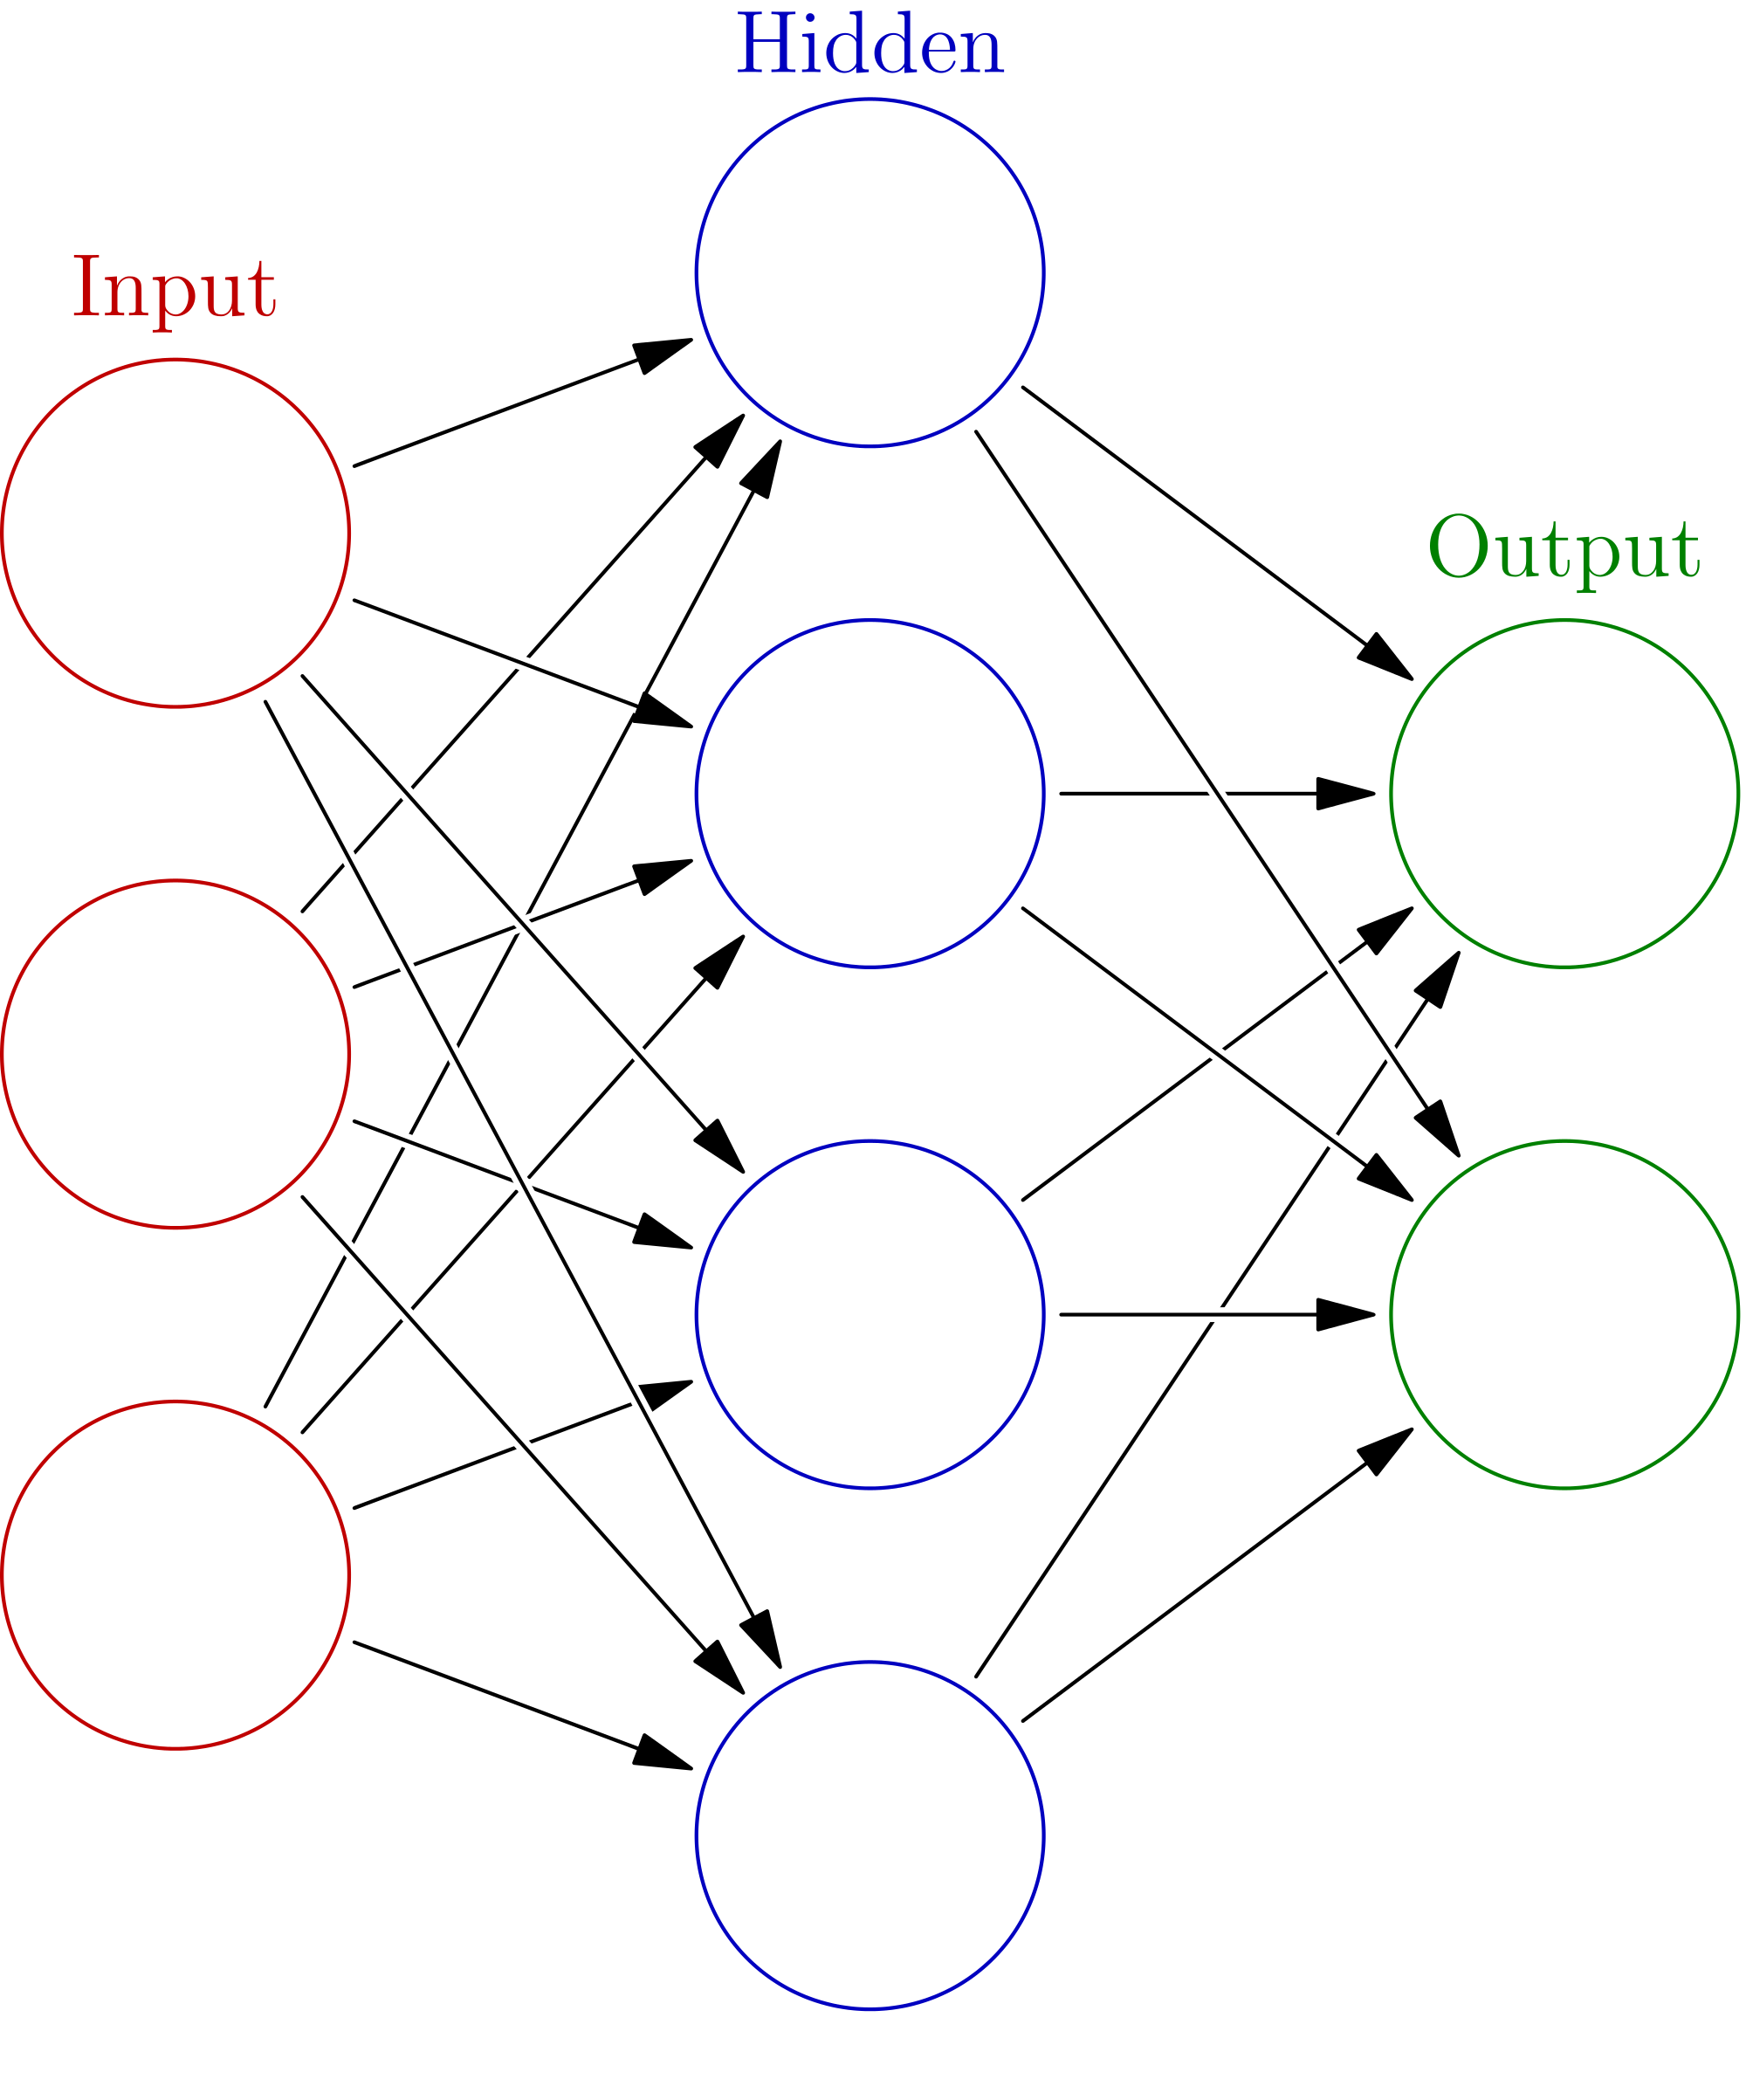
\includegraphics[width=0.5\textwidth]{NN.png}
			\caption{Artificial neural network}
			\label{NN}
		\end{figure}
		
		For this experiment a neural network with single hidden layer was used. The features used for the Neural Network are as shown in Table \ref{NN_features}.
		\begin{table}[h!]
			\centering
			\caption{Neural Network Features}
			\label{NN_features}
			\begin{tabular}{l l}
				\hline
				Parameters &Value\\\hline
				Type of network &Radial Basis Function(RBF) network\\
				Input layer size &8\\
				No. of hidden layers &1\\
				Hidden layer size &8\\
				Activation function in hidden layer &Sigmoid\\
				Optimization function &fmincg\\
			\end{tabular}
		\end{table}
		The training set is used to train the Neural Network to obtain the network parameters (Thetas). The testing set is then passed through the trained neural network to obtain the classes to which the testing data belongs to.
	\subsection{Support Vector Machines (SVM)}
		Support vector machines (SVM) are one of the supervised learning models used in machine learning. SVMs can perform both linear and non-linear classification. Non-linear classification is done using kernel method, where inputs are mapped into higher dimensional feature vectors. The classification boundary obtained using SVMs have a special property, i.e, the boundary has the largest distance from the nearest training data point of any class. SVMs are suitable for binary classification. However, multi-class classification can be done using one-vs-all method. In one-vs-all classification method, a series of binary classifiers are built which distinguish between one label and the rest and classes are assigned using winner-takes-it-all strategy.
		
\section{Results}
	
	\subsection{Intra-Subject Classification}
		Classification accuracies for various combinations of the classes were calculated. Two class classification accuracies using the data sets for calculation and breathing of different test subjects are shown in Table \ref{ICB}.  
		\begin{table}[h!]
			\centering
			\caption{Intra-subject, Calculation-Breathing Classification}
			\label{ICB}
			\begin{tabular}{c c c c}
				\hline
				Sub &Mahalanobis &Neural Net &SVM\\\hline
				1 &68.67 &77.67 &80.00\\
				2 &68.67 &70.33 &73.67\\
				3 &60.00 &73.33 &69.67\\
				4 &68.67 &77.00 &77.67\\
			\end{tabular}
		\end{table}
		Similarly, two class classification accuracies using the data sets for calculation and singing of different test subjects are shown in Table \ref{ICS}.
		\begin{table}[h!]
			\centering
			\caption{Intra-subject, Calculation-Singing Classification}
			\label{ICS}
			\begin{tabular}{c c c c}
				\hline
				Sub &Mahalanobis &Neural Net &SVM\\\hline
				1 &60.67 &68.67 &69.00\\
				2 &68.33 &50.67 &71.67\\
				3 &59.00 &57.67 &64.00\\
				4 &76.67 &78.00 &86.67\\
			\end{tabular}
		\end{table}
		Also, two class classification accuracies using the data sets for breathing and singing of different test subjects are shown in Table \ref{IBS}.
		\begin{table}[h!]
			\centering
			\caption{Intra-subject, Breathing-Singing Classification}
			\label{IBS}
			\begin{tabular}{c c c c}
				\hline
				Sub &Mahalanobis &Neural Net &SVM\\\hline
				1 &55.00 &66.33 &58.67\\
				2 &69.67 &67.67 &76.00\\
				3 &62.67 &68.67 &72.67\\
				4 &66.33 &70.33 &76.33\\
			\end{tabular}
		\end{table}
 		Finally, three class classification accuracies using the data sets for calculation, breathing and singing of different subjects are shown in Table \ref{ICBS}.
		\begin{table}[h!]
			\centering
			\caption{Intra-subject, Calculation-Breathing-Singing Classification}
			\label{ICBS}
			\begin{tabular}{c c c c}
				\hline
				Sub &Mahalanobis &Neural Net &SVM\\\hline
				1 &46.67 &52.44 &54.00\\
				2 &55.78 &45.33 &58.89\\
				3 &44.67 &47.56 &45.33\\
				4 &57.56 &56.89 &64.22\\
			\end{tabular}
		\end{table}
	\FloatBarrier
	\subsection{Inter-Subject Classification}
		Table \ref{In12} shows the 2 class classification accuracies for just 2 test subjects. Similarly, Table \ref{In123} shows the 3 class classification accuracies for just 3 test subjects. Finally, Table \ref{In1234} shows the 4 class classification accuracies for all the 4 test subjects.
		\begin{table}[h!]
			\centering
			\caption{Inter-subject Classification for just subject 1 and 2}
			\label{In12}
			\begin{tabular}{c c c c}
				\hline
				Task &Mahalanobis &Neural Net &SVM\\\hline
				Calculation &83.33 &85.67 &92.33\\
				Breathing &66.00 &68.00 &76.33\\
				Singing &75.67 &84.33 &88.67\\
			\end{tabular}
		\end{table}
		
		\begin{table}[h!]
			\centering
			\caption{Inter-subject Classification for subjects 1,2 and 3}
			\label{In123}
			\begin{tabular}{c c c c}
				\hline
				Task &Mahalanobis &Neural Net &SVM\\\hline
				Calculation &71.56 &81.11 &82.00\\
				Breathing &57.33 &56.89 &58.89\\
				Singing &68.00 &71.78 &73.56\\
			\end{tabular}
		\end{table}
		
		\begin{table}[h!]
			\centering
			\caption{Inter-subject Classification for all 4 subjects}
			\label{In1234}
			\begin{tabular}{c c c c}
				\hline
				Task &Mahalanobis &Neural Net &SVM\\\hline
				Calculation &70.00 &79.00 &73.33\\
				Breathing &58.67 &54.67 &56.17\\
				Singing &65.33 &68.67 &67.33\\
			\end{tabular}
		\end{table}
		\FloatBarrier

\section{Observations}
	\begin{enumerate}
		\item Classification accuracies for both intra and inter subject tests are generally high for Neural Networks and SVMs compared to Mahalanobis Distance. This may be due to the assumption of the data being normal distribution which might be false. The data actually failed the Henze-Zirkler's Multivariate Normality Test.

		\item The intra-subject classification accuracies are less compared to inter-subject classification accuracies. This might be due to similarities in the EEG data for a particular subject.

		\item For intra-subject case, the classification accuracies are higher for the tests involving calculation task, indicating the EEG data for the calculation task can be very well separated from other tasks.

		\item For inter-subject case, the classification accuracies drop as we increase the number of test subjects.

		\item We can harness the above methods for verification use case. This can be done by seeing which subject class is classified maximum times for a given test subject in a given interval.
	\end{enumerate}


\section{Future Work}
	\begin{enumerate}
		\item Explore methods which can used for user verification.
		\item Explore online learning.
		\item Explore methods to improve the classification accuracies.
	\end{enumerate}


\end{document}  